\section{Simulation Analysis}
\label{sec:simulation}

\subsection{AC/DC Converter Simulation}
\label{subsec:circuit_simulation}
\par In this section we simulate an AC/DC COnverter for 10 periods. It is our goal to understand how the values of each component affects the precision and the quality of the output voltage. This circuit transforms a variable voltage into a voltage with a DC component as closest as one can get to the pretended value, reducing, at the same time, the oscilation around that value. In order to do it we used the values indicated in the begginig of Section \ref{sec:analysis}.

\par  \textbf{Important note:} Beyond modelling and analysing the circuit provided, one of the goals of this laboratory assignment is to maximize the merit, which is computed according to the following formula:
\begin{equation}
M = \frac{1}{\text{cost}*[\text{ripple}(v_0)+\text{average}(v_{0}-12)+10^{-6}]}
\end{equation}

Therefore, it was our intention to obtain the best value for this parameter,using each of the variables in order to maximize it, wich means that we have not tried to improve each of those separately, but as a all. 


\subsection{Output Voltage Level and Ripple}
\label{subsec:out_voltage}
In order to measure the output voltage level, we have used Ngspice's \textit{average} function to determine its mean value. Beyond that it was from our interest to determine the ripple on the voltage. To do it, we have used Ngspice's \textit{max} and \textit{min} functions, which have allowed us to compute the amplitude of the oscilation. The results obtained are shown in the table bellow:


\begin{table}[H]
  \centering
  \begin{tabular}{|l|r|}
    \hline    
    {\bf Name} & {\bf Value [A or V]} \\ \hline
    gib[i] & 6.327120e-18\\ \hline
r1[i] & -6.04063e-18\\ \hline
r2[i] & 6.327120e-18\\ \hline
r3[i] & 2.864858e-19\\ \hline
r4[i] & 1.289989e-18\\ \hline
r5[i] & -2.78376e-03\\ \hline
r6[i] & 1.301043e-18\\ \hline
r7[i] & 2.625374e-18\\ \hline
v(1) & 0.000000e+00\\ \hline
v(2) & 6.197538e-15\\ \hline
v(3) & 1.898958e-14\\ \hline
v(4) & -2.62707e-15\\ \hline
v(5) & 5.329071e-15\\ \hline
v(6) & 8.618561e+00\\ \hline
v(7) & -2.62707e-15\\ \hline
v(8) & -5.32907e-15\\ \hline

  \end{tabular}
  \caption{Operating point. A variable followed by [i] or [current] is of type {\em current}
    and expressed in Ampere; other variables are of type {\it voltage} and expressed in
    Volt.}
  \label{tab:out_voltage}
\end{table}



\newpage
\subsection{Envelope Detector and Voltage Regulator - Output Voltages and Ripple}

\par In this section, it is presented the plots regarding both envelope detector and voltage regulator output voltages and ripple.
The values for each one of this 'subcircuits' are shown in the following tables:

\begin{table}[H]
  \centering
  \begin{tabular}{|l|r|}
    \hline    
    {\bf Name} & {\bf Value [A or V]} \\ \hline
    gib[i] & 6.327120e-18\\ \hline
r1[i] & -6.04063e-18\\ \hline
r2[i] & 6.327120e-18\\ \hline
r3[i] & 2.864858e-19\\ \hline
r4[i] & 1.289989e-18\\ \hline
r5[i] & -2.78376e-03\\ \hline
r6[i] & 1.301043e-18\\ \hline
r7[i] & 2.625374e-18\\ \hline
v(1) & 0.000000e+00\\ \hline
v(2) & 6.197538e-15\\ \hline
v(3) & 1.898958e-14\\ \hline
v(4) & -2.62707e-15\\ \hline
v(5) & 5.329071e-15\\ \hline
v(6) & 8.618561e+00\\ \hline
v(7) & -2.62707e-15\\ \hline
v(8) & -5.32907e-15\\ \hline

  \end{tabular}
  \caption{Operating point. A variable followed by [i] or [current] is of type {\em current}
    and expressed in Ampere; other variables are of type {\it voltage} and expressed in
    Volt.}
  \label{tab:out_voltage2}
\end{table}


\begin{table}[H]
  \centering
  \begin{tabular}{|l|r|}
    \hline    
    {\bf Name} & {\bf Value [A or V]} \\ \hline
    gib[i] & 6.327120e-18\\ \hline
r1[i] & -6.04063e-18\\ \hline
r2[i] & 6.327120e-18\\ \hline
r3[i] & 2.864858e-19\\ \hline
r4[i] & 1.289989e-18\\ \hline
r5[i] & -2.78376e-03\\ \hline
r6[i] & 1.301043e-18\\ \hline
r7[i] & 2.625374e-18\\ \hline
v(1) & 0.000000e+00\\ \hline
v(2) & 6.197538e-15\\ \hline
v(3) & 1.898958e-14\\ \hline
v(4) & -2.62707e-15\\ \hline
v(5) & 5.329071e-15\\ \hline
v(6) & 8.618561e+00\\ \hline
v(7) & -2.62707e-15\\ \hline
v(8) & -5.32907e-15\\ \hline

  \end{tabular}
  \caption{Operating point. A variable followed by [i] or [current] is of type {\em current}
    and expressed in Ampere; other variables are of type {\it voltage} and expressed in
    Volt.}
  \label{tab:out_env}
\end{table}

Next, we present the plot regarding the results obtained:

\begin{figure}[H] \centering
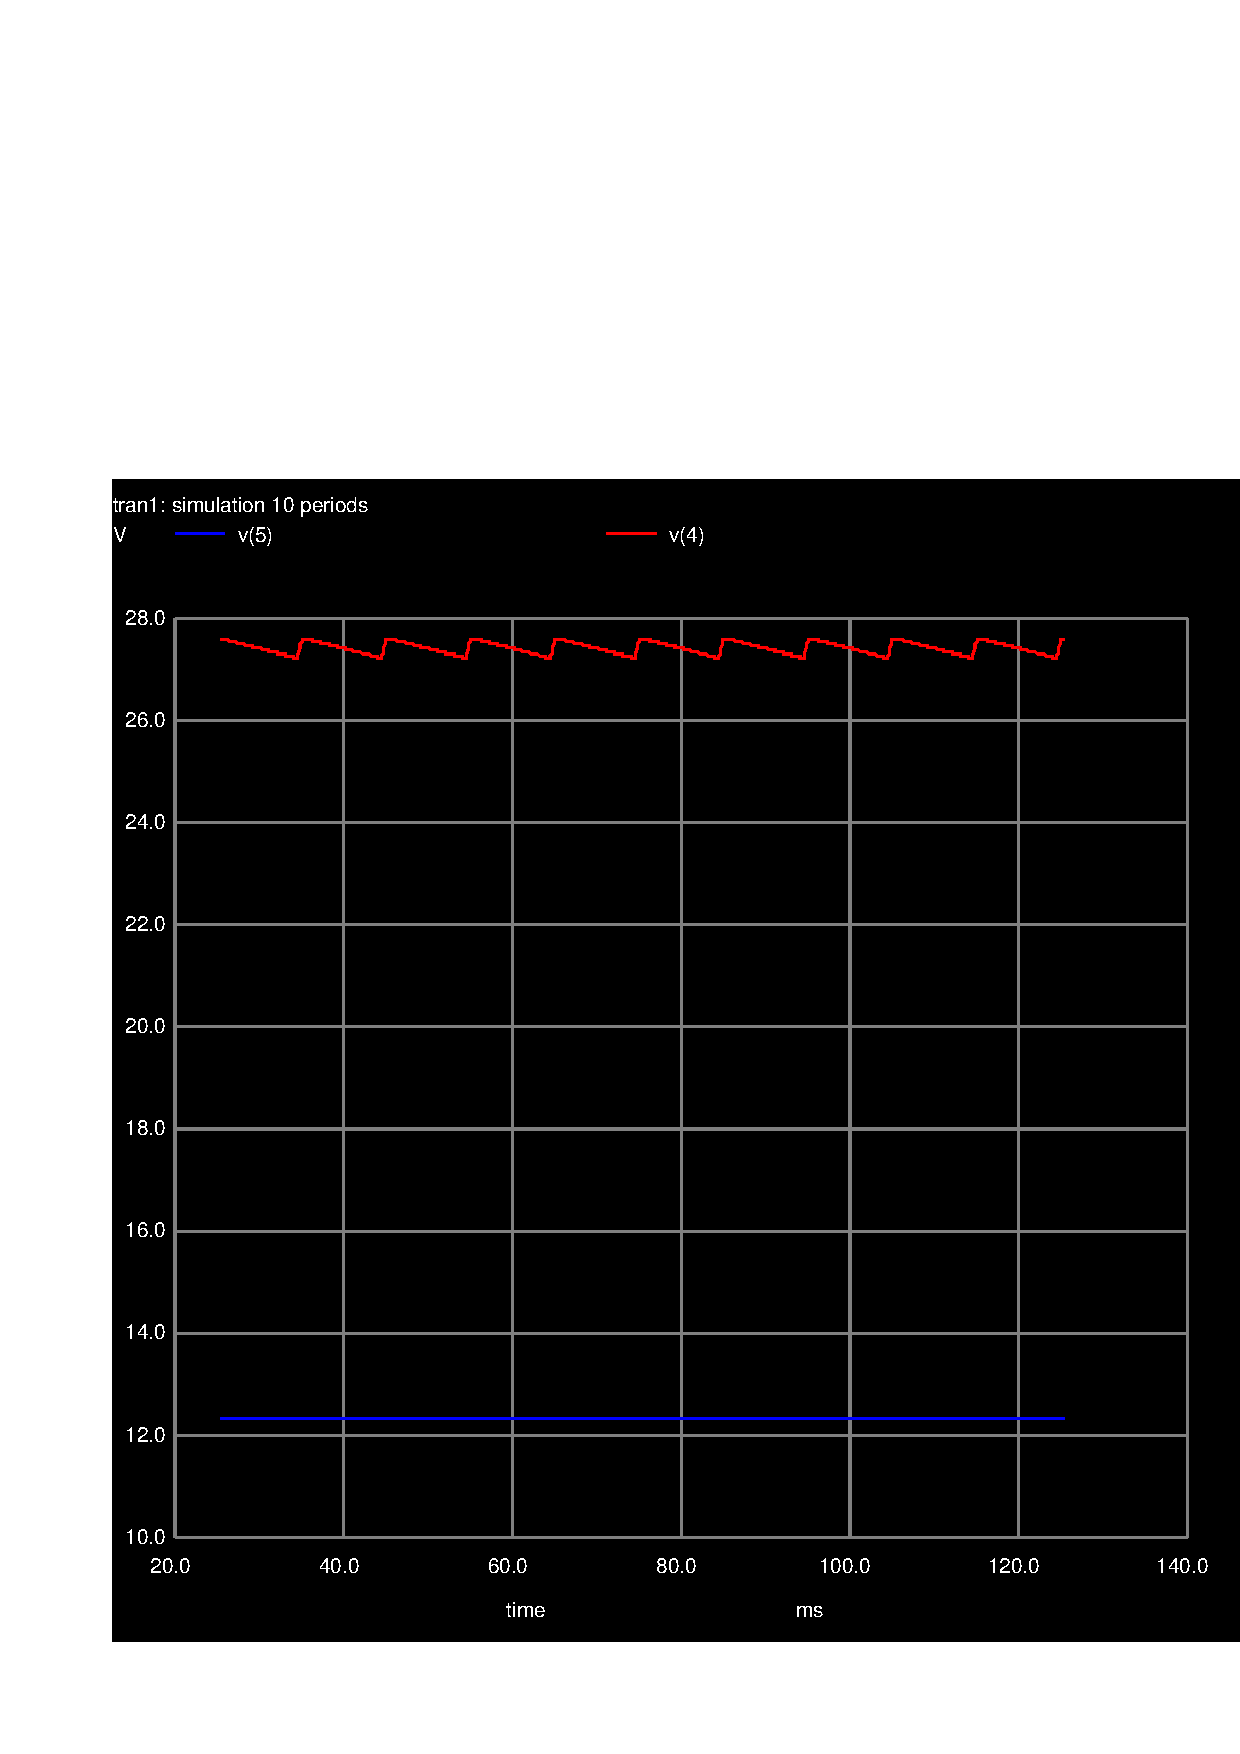
\includegraphics[clip, trim=1.3cm 1.3cm 0cm 7cm, width=0.6\linewidth]{ende.pdf}
\caption{Total solution of the voltage source and the capacitor}
\label{fig:env+vore}
\end{figure}


As one can conclude from the plot analysis, the ripple suffers a significant reduction from the envelope detector to the the voltage regulator. This last circuit has the same output voltage as the ac/dc converter as a all. That is why table \ref{tab:out_voltage2} is equal to table \ref{tab:out_voltage} in Subsection \ref{subsec:circuit_simulation}.



\subsection{Final Result}

\par As mentioned in Subsection \ref{subsec:circuit_simulation} our goal is to obtain a voltage as stable as possible as well as closest as possible to 12V. Therefore, in this subsection we present a plot where the difference beetwen the output voltage and the pretended result is shown.

\begin{figure}[H] \centering
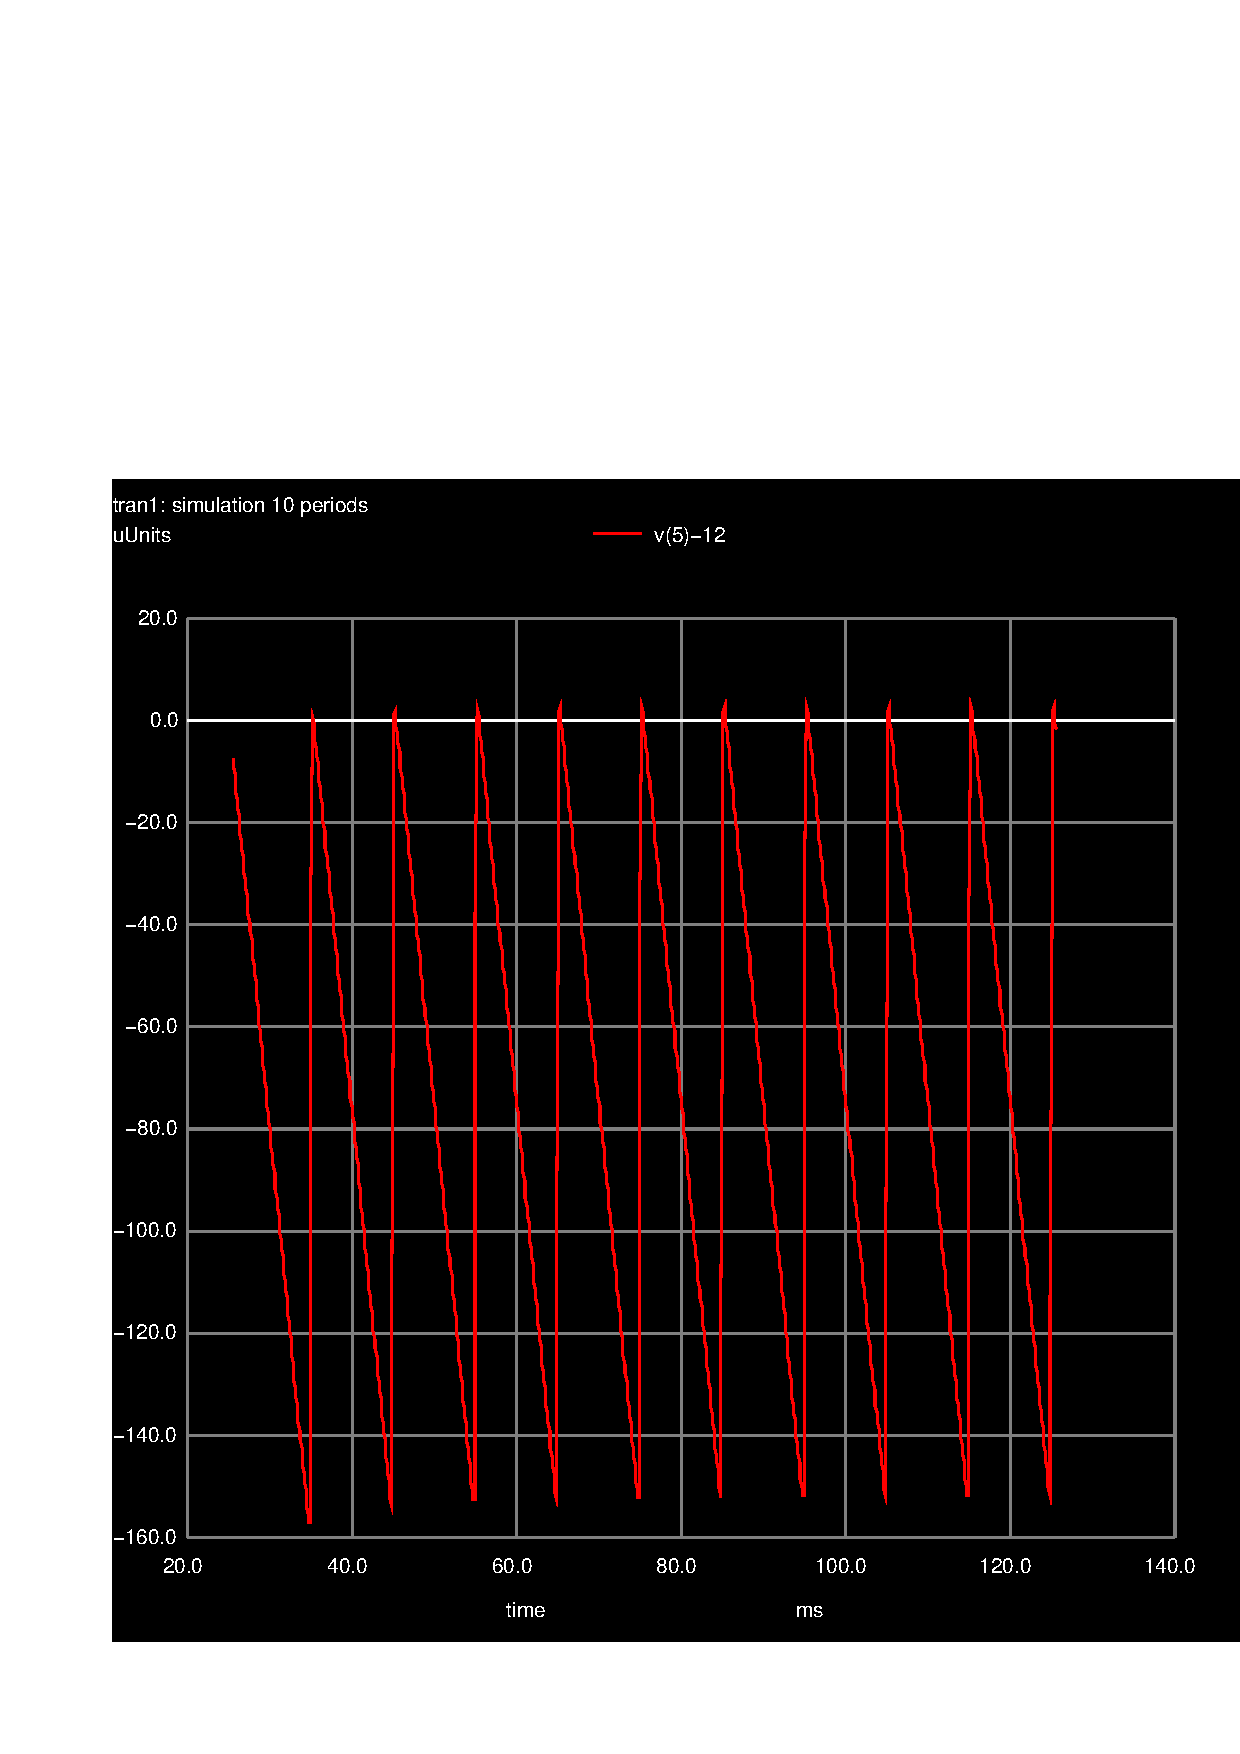
\includegraphics[clip, trim=1.3cm 1.3cm 0cm 7cm, width=0.6\linewidth]{deviation.pdf}
\caption{Total solution of the voltage source and the capacitor}
\label{fig:vo-12}
\end{figure}


As one can see, we were able to complete this laboratory objective, since we ended up with a voltage which as a DC component really close to 12V and with a minimum AC component.



